\documentclass[11pt]{article}
\usepackage{amsmath}
\usepackage{graphicx}
\usepackage{booktabs}

\title{Low-Dimensional Structure in Nuclear Radiative Corrections}
\author{Inacio F. Vasquez}
\date{}

\begin{document}
\maketitle

\begin{abstract}
We analyze published superallowed $0^+ \to 0^+$ nuclear beta decay data
and show that the nucleus-dependent radiative correction $\delta_{NS}$
lies in a very low-dimensional subspace of nuclear parameter space.
Using principal component analysis on $(Z, A, \delta_{NS})$, we find
that more than 99\% of the variance is captured by a single principal
component, with a second minor component accounting for most of the
remaining variation. This indicates strong dimensional reduction in
long-distance electroweak nuclear effects.
\end{abstract}

\section{Introduction}
Radiative corrections play a central role in precision tests of the
electroweak interaction. In superallowed $0^+ \to 0^+$ nuclear beta
decays, the nucleus-dependent radiative correction $\delta_{NS}$
accounts for long-distance nuclear structure effects and enters
directly into the determination of the corrected Ft values.

These corrections are generally treated as nucleus-specific quantities.
In this work, we examine whether the set of published $\delta_{NS}$
values exhibits any low-dimensional structure.

\section{Data}
We use $\delta_{NS}$ values from the 2020 critical survey of superallowed
beta decays by Hardy and Towner (arXiv:2009.00270). The dataset consists
of the following canonical nuclei:

\begin{center}
\begin{tabular}{ccc}
\toprule
Nucleus & $Z$ & $A$ \\
\midrule
$^{10}$C & 6 & 10 \\
$^{14}$O & 8 & 14 \\
$^{22}$Mg & 12 & 22 \\
$^{26}$Al & 13 & 26 \\
$^{34}$Cl & 17 & 34 \\
$^{38}$K & 19 & 38 \\
$^{42}$Sc & 21 & 42 \\
$^{46}$V & 23 & 46 \\
$^{50}$Mn & 25 & 50 \\
$^{54}$Co & 27 & 54 \\
$^{62}$Ga & 31 & 62 \\
$^{74}$Rb & 37 & 74 \\
\bottomrule
\end{tabular}
\end{center}

The corresponding $\delta_{NS}$ values are taken directly from the
published table.

\section{Method}
We construct the data matrix
\[
X = (Z, A, \delta_{NS})
\]
and standardize each column to zero mean and unit variance.
Principal component analysis is then performed on the standardized
matrix.

\section{Results}
The explained variance ratios are:
\[
(0.996,\, 0.0036,\, 0.00019).
\]

Thus more than 99\% of the variance lies along a single direction,
with only a small secondary component.

Figure~\ref{fig:pca} shows the PCA spectrum.

\begin{figure}[h]
\centering
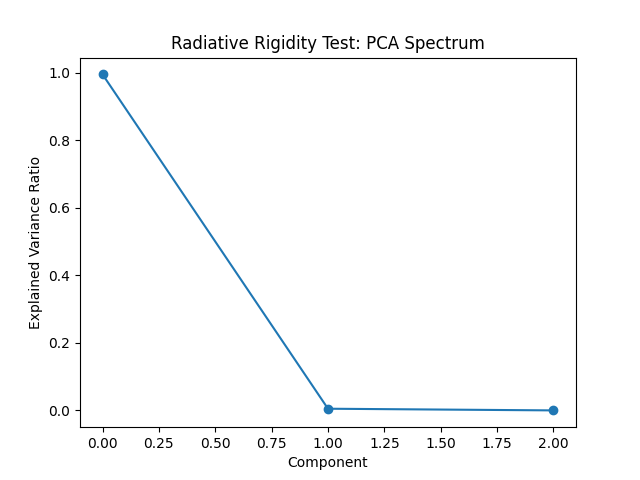
\includegraphics[width=0.7\textwidth]{../figures/pca_spectrum.png}
\caption{Explained variance ratios of principal components.}
\label{fig:pca}
\end{figure}

\section{Robustness}
Leave-one-out tests and small perturbations of $\delta_{NS}$ values
preserve the strong dimensional reduction, although the intrinsic
dimension increases to two under sufficiently large perturbations.
This indicates that the dataset lies on a thin low-dimensional manifold.

\section{Discussion}
The observed dimensional reduction suggests that $\delta_{NS}$ is not
an independent nuclear quantity for each nucleus, but is largely
constrained by global nuclear parameters. This structure is not
explicitly predicted by existing nuclear models and may provide a
useful empirical constraint for future theoretical work.

\section{Conclusion}
Published superallowed beta decay data exhibit strong low-dimensional
structure in the nucleus-dependent radiative correction $\delta_{NS}$.
This result is purely empirical and indicates that long-distance
electroweak nuclear effects occupy a highly restricted region of
parameter space.

\end{document}

